\documentclass[12pt,a4paper]{article}
\usepackage{lipsum}
\usepackage{authblk}
\usepackage[marginparwidth=2in,top=2cm, bottom=2cm, left=1cm, right=2.5in]{geometry}

\PassOptionsToPackage{hyphens}{url}
\usepackage{hyperref}

\usepackage{multicol}
\usepackage{textcomp}
\usepackage{color}
\usepackage{graphicx}
\definecolor{pblue}{rgb}{0.13,0.13,1}
\definecolor{pgreen}{rgb}{0,0.5,0}
\definecolor{pred}{rgb}{0.9,0,0}
\definecolor{pgrey}{rgb}{0.46,0.45,0.48}

\newcommand{\lectnote}[1]{\marginpar{\texttt{{\small{ #1 } }}}}

\usepackage{listings}
\lstdefinestyle{term}{language=bash,
  columns=fullflexible,
  showspaces=false,
  showtabs=false,
  breaklines=true,
  showstringspaces=false,
  tabsize=2,
  breakatwhitespace=true,
  commentstyle=\color{pgreen},
  keywordstyle=\color{pblue},
  stringstyle=\color{pred},
  basicstyle=\small\ttfamily,
  frame=single,
  moredelim=[il][\textcolor{pgrey}]{$$},
  moredelim=[is][\textcolor{pgrey}]{\%\%}{\%\%},
  upquote=true
}
\lstdefinestyle{sh}{language=bash,
  columns=fullflexible,
  showspaces=false,
  showtabs=false,
  breaklines=true,
  showstringspaces=false,
  tabsize=2,
  breakatwhitespace=true,
  commentstyle=\color{pgreen},
  keywordstyle=\color{pblue},
  stringstyle=\color{pred},
  numbers=left,
  stepnumber=1,
  basicstyle=\small\ttfamily,
  frame=single,
  moredelim=[il][\textcolor{pgrey}]{$$},
  moredelim=[is][\textcolor{pgrey}]{\%\%}{\%\%},
  upquote=true
}

\lstdefinestyle{py}{language=python,
  columns=fullflexible,
  showspaces=false,
  showtabs=false,
  breaklines=true,
  showstringspaces=false,
  tabsize=2,
  breakatwhitespace=true,
  commentstyle=\color{pgreen},
  keywordstyle=\color{pblue},
  stringstyle=\color{pred},
  numbers=left,
  stepnumber=1,
  basicstyle=\small\ttfamily,
  frame=single,
  moredelim=[il][\textcolor{pgrey}]{$$},
  moredelim=[is][\textcolor{pgrey}]{\%\%}{\%\%},
  upquote=true
}

\lstdefinestyle{txt}{
  columns=fullflexible,
  showspaces=false,
  showtabs=false,
  breaklines=true,
  showstringspaces=false,
  tabsize=2,
  breakatwhitespace=true,
  numbers=left,
  stepnumber=1,
  basicstyle=\small\ttfamily,
  frame=single,
  moredelim=[il][\textcolor{pgrey}]{$$},
  moredelim=[is][\textcolor{pgrey}]{\%\%}{\%\%},
  upquote=true
}

\usepackage[T1]{fontenc}

\newcommand{\schedule}[2]{\textbf{#1} \textit{#2}}

\usepackage{fancyhdr}
%
\pagestyle{fancy}
%
\renewenvironment{abstract}{%
\hfill\begin{minipage}{0.95\textwidth}
\rule{\textwidth}{1pt}}
{\par\noindent\rule{\textwidth}{1pt}\end{minipage}}
%
\makeatletter
\renewcommand\@maketitle{%
\hfill

\begin{minipage}{0.95\textwidth}
\vskip 1em
\let\footnote\thanks 
{\LARGE \@title \par }
\vskip 0.5em
{\large \@author \par}
\vskip 0.5em
{\large \@date \par}
\end{minipage}
\vskip 1em \par
}

\makeatother
%
\begin{document}
%
%title and author details
\title{\textbf{cron, tar, SQL, and exam}}
\author[1]{Melvyn Ian Drag}
\date{\today}
%
\maketitle
%
\begin{abstract}
In this lecture you'll learn cron, how to backup your linux machine, a bit about
SQL ( not essential, but should help you get more out of next week's lecture )
and then we'll discuss the exam a bit.
\end{abstract}

\section{Introduction}
Plan for the evening:
\begin{itemize}
\setlength\itemsep{0em}
\item \schedule{7:00 - 7:20}{get setup}
\item \schedule{7:20 - 7:30}{morale boosting review}
\item \schedule{7:30 - 7:55}{backups with cron + tar}
\item \schedule{7:55 - 8:00}{Break}
\item \schedule{8:00 - 9:00}{sqlite3 murder mystery}
\item \schedule{9:00 - 9:05}{Break}
\item \schedule{9:05 - 9:45}{prepare for exam}
\end{itemize}

\section{Setup}

Create a NEW \$5 Debian 10 server and add your ssh key so you can get in.

{\LARGE MAKE SURE ITS A FRESH NEW SERVER! }

Then:
\begin{lstlisting}[style=term]
root@machine$ apt update
root@machine$ apt install sqlite3 # well use this later.
root@machine$ git clone https://github.com/melvyniandrag/LinuxClassRepo.git
#\end{lstlisting}

\section{Review}

At this point, we're 7 weeks ( nearly 2 months! ) into your Linux career. You
may be realizing that learning Linux is something of a lifestyle - this will
take lots of practice! Soon we'll start doing some real projects on our Linux
machines like configuring various types of servers, but let's make sure that we
know basic things like create files, move and modify files, and navigate our
linux machine with ease.
 I expect you to understand these concepts right
now:\marginpar{\texttt{{\small should use this right margin for lecturer notes - what to draw on
the board, what leading questions to ask students, relevant anecdotes, etc.}}}
\begin{enumerate}
\setlength\itemsep{0em}
\item create a hidden file
\item create a directory
\item delete a file
\item delete a directory
\item add some text to a file with vim.
\item what are some text editors besides vim?
\item why are we using vim in this class and not those ( answer : I like vim and
it's my class. If you like nano or pico or emacs, then use that on your own
time! In this class we're learning vim.
\item ls
\item ls -a
\item ls -l
\item chmod
\item How to execute a file with "./"
\item cp
\item cp -r
\item mkdir -p
\item mv
\item rm 
\item rm -r
\item what's the sudo group?
\item who is root?
\item how to install software on debian with apt?
\end{enumerate}

There's more to know, I just spent a minute thinking about the semester - the
definitive source of what you should know is in the lecture materials from the
previous six weeks.

\section{cron}
\textbf{cron} is used for scheduling jobs on your computer. You can modify a
thing called a \textbf{crontable} to tell your computer to do thing at certain time(s) in the future.

All you have to do is add some command(s) to the crontable and then yuou're good
to go! The computer will do the rest of the work! Pretty cool stuff. Your phone
does stuff like this already - What'sApp usually backs up your messages and
images to the cloud at night time, I don't know what Google Photos and iCloud
do, but they probably do something similar or offer you a mechanism to do  it.

We are using vim in this class, so we'll want to make sure that the crontable is
opened with vim. Make sure to perform the following step to set your default
editor to vim.

\begin{lstlisting}[style=term]
# note I haven't tested this command yet,
# make sure I've written it right please, students!
# I don't have internet now and i'm just going by memory
root@digitalOcean$ apt install vim
root@digitalOcean$ update-alternatives --config editor
# then choose vim or vi
# if you have multiple choices for vim, choose vim.basic
\end{lstlisting}

Now we are ready.

View your cron table with \textit{crontab -l}, edit the crontab with \textit{crontab -e}.
Choose vim if prompted to  select which text editor to use. It may say vim.tiny,
vim.basic. To be honest in all these years I've just chosen a random one. I
should learn the distinction.

To schedule jobs, you add rows of the form
\begin{lstlisting}
m h dom moy dow command
\end{lstlisting}

where the above represent:

\begin{itemize}
\item m - minute (0-59),
\item h - hour (0-23),
\item dom - day of the month (1-31),
\item moy - month of the year (1-12),
\item dow - day of the week (0-6, 0=Sunday)
\item command - bash command
\end{itemize}

For example, to echo "hello" into a file on March 4th, every minute of the 19th
hour of the day, you will add the following line to your crontab, as the root
user. \lectnote{Maybe belabor this point a bit. The m h dom etc. stuff can be
confusing at first. Take a few minutes to discuss it with students to try and
clarify it a bit.}

\begin{lstlisting}[style=sh]
* 19 4 3 * echo "hello" >> /root/hello.txt
\end{lstlisting}

Note that the above command says * for minutes ( aka any minute ) 19 for hours (
if the hour is 19 ), 4 for day ( if the date of the month is 4 ), 3 for month (
March ) and * for dow ( any day of the week, could be monday, tuesaday, etc. ).

You will note that these conditions are all met right now, today! If you add
this to your crontab and wait a few minutes, then look at /root/hello.txt,
you'll see it says ``hello'' a few times inside!

So now you know how to schedule jobs on your computer. See figure
~\ref{fig:cronOnLaptop} to see me running the above cronjob on my computer. 

\begin{figure}[h]
\centering
	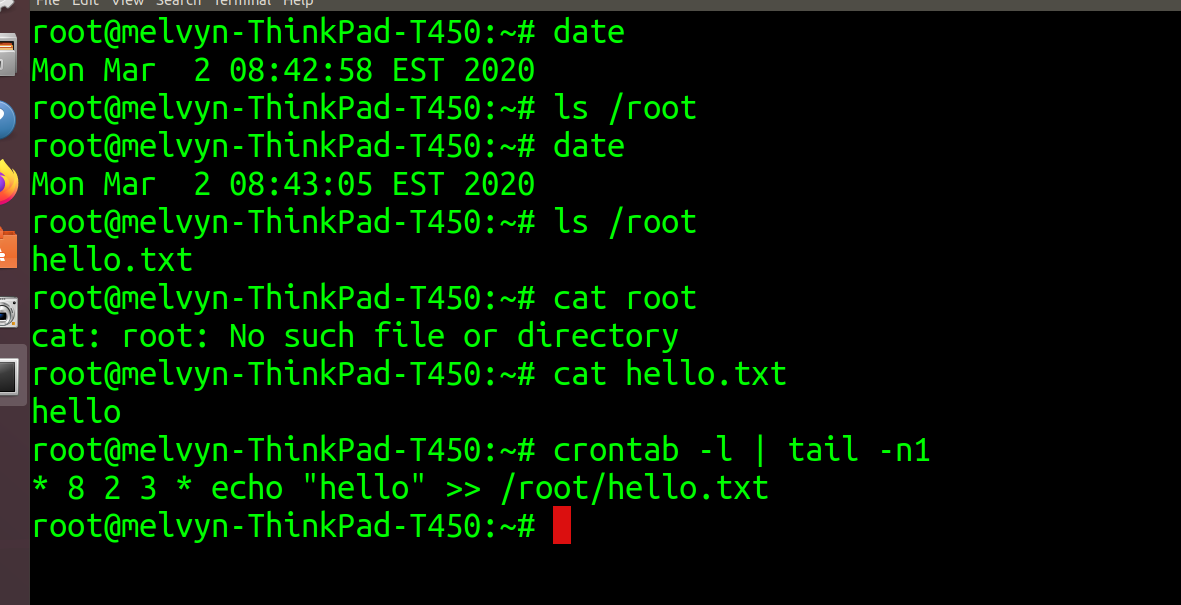
\includegraphics[width=0.8\textwidth]{Images/cronOnLaptop.png}
	\caption{{\small \texttt{Check the timestamps! There was not file called /root/hello.txt,
but then magically a minute later it was there. In the image I show you my
crontable entry.}}}
	\label{fig:cronOnLaptop}
\end{figure}

\section{Backups with Cron}
This was a silly example that I just gave you. More commonly you'll use cron to
back up your computer.

\subsection{tar}
\textbf{tar} is used for creating archives, i.e. a single file containing a bunch of
files. It's similar to a zip or rar file you may have seen at some time in your
life. Heck, you may be using tar files everyday too, I don't know. Some folks
were submitting me homeworks in the beginning of class as an archive - I can't
remember if people were submitting zips, tars or what. In any event, let's
create a little sample directory  and we'll use tar to pack it into an archive.


For the example I created the files / directories shown in figure
~\ref{fig:tarExample1}

\begin{figure}[h]
\centering
	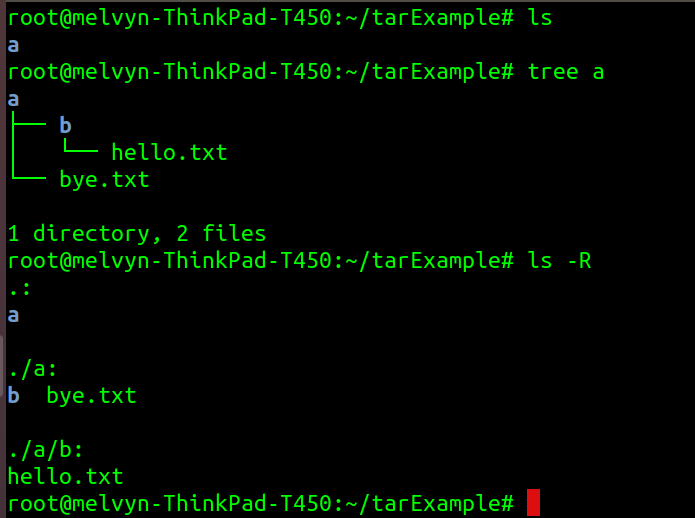
\includegraphics[width=0.8\textwidth]{Images/tarExample1.png}
	\caption{{\small \texttt{Files for this example. There is nothing special about these files
and directories, we're just using them for the example. Also note I'm showing
two ways to view files in directories - \textit{tree} and \textit{ ls -R}}}}
	\label{fig:tarExample1}
\end{figure}


Now what I want to do now is create a tar archive from these files. Here's how
you do it:

\begin{lstlisting}[style=term]
root@machine$ ls
a
root@machine$ tar -cvf a.tar a # create a.tar from directory a. 
root@machine$ ls 
a a.tar
\end{lstlisting}

To verify that it worked, let's unpack the archive in another directory.

\begin{lstlisting}[style=term]
root@machine$ ls
a a.tar
root@machine$ mkdir NewDirectory
root@machine$ mv a.zip NewDirectory
root@machine$ cd NewDirectory
root@machine$ ls
a.tar
root@machine$ tar -xvf a.tar
root@machine$ ls
a.tar a 
\end{lstlisting}

In the above examples you've seen how to create a .tar archive and how to unpack
it. For the record, let's just see where the tar executable is on our system:

\begin{lstlisting}[style=term]
root@machine$ which tar
/usr/bin/tar
\end{lstlisting}

This output may vary. It might say `/bin/tar' or `/usr/bin/tar' or something
else. This doesn't matter. Just make a mental note of what it says.

\subsection{backup}

I already showed you a cron job using echo. Now we'll just do a cronjob with
tar. A subtle and important difference between tar and echo is that echo is a
builtin command, and tar is not. If you are dying to know what that means, or
finding my class too easy, then ask me after class and I'll explain the
differnce. What matters to you and your grade, is that you are able to create a
cron job with tar. And here is how you do it:

In this example, we will back up /home/yourname to a tar file. There are many
ways to do this, but I'm going to show you this way to give your fingers some
practice. To learn more about this, go on youtube, or talk to me when we both
have free time. 

Create a user for the coming example:

\begin{lstlisting}[style=term]
root@machine$ adduser YOURNAMEHERE
# then follow the instructions as last time
\end{lstlisting}

Add the following line to root's crontab to back up /home/melvyn every day at
midnight.

NOTE: BELOW I PUT /USR/BIN/TAR - you need to put the output of `which tar'. I
don't know where tar will be on your system. \lectnote{Change the cron schedule
to one that will be useful in class so students can see it in action. The time
is probably around 7:40 pm. So set the time stamp to 42 19 * * * so that the tar
command will run at 7:42 PM.}

\begin{lstlisting}
0 0 * * * /usr/bin/tar -cvf /root/melvyn-home.tar /home/melvyn
\end{lstlisting}

AND OF COURSE YOU MUST HAVE CREATED A USER `melvyn' for this to work otherwise
there won't be any /home/melvyn to backup.

\subsection{Going Further}
That's all you need to know to get started! If you want to go further you might
want to know what happens if a cronjob fails. Whenever cron has output, be it
error output or standard output, it wants to email you. You'll see a message in
/var/log/syslog that looks like what I'm showing in figure ~\ref{fig:mta}

\begin{figure}[h]
\centering
	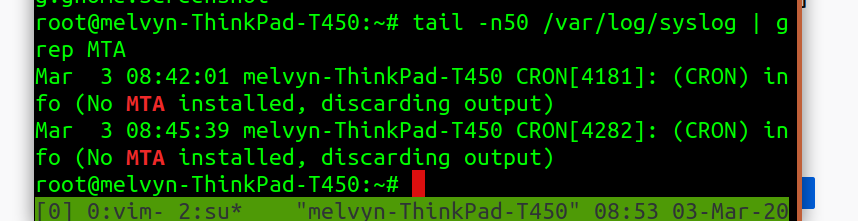
\includegraphics[width=0.8\textwidth]{Images/cronOutput.png}
	\caption{{\small \texttt{cron wants to send you emails telling you about your cron jobs. If
you want to configure your machine to email you the status of your cron jobs,
google `MTA', `cron' and `postfix' and follow a tutorial.}}}
	\label{fig:mta}
\end{figure}

Also, you might want to know that .tar does not compress your files - it only
creates an archive. It puts them all into a big box. But they aren't squished.
So, if you have 1GB of files and you create a .tar from them - you'll have a
.tar that's bigger than 1GB, because it has to contain all the uncompressed
stuff plus some data specific to tar files. If you want to compress your files,
try adding the -z option to your compression command, and name the file .tar.gz.
Like this:

\begin{lstlisting}[style=term]
user@machine$ tar -xvzf compressedArchive.tar.gz directoryToCompress
\end{lstlisting}

Compression is an interesting topic, very important and lots to say about it,
but we have a schedule to keep! If you're enjoying this class and don't feel
like you're drowning, then definitely go google about .gz files or come talk to
me about it or whatever.

Moving on, now we'll plant some seeds of knowledge that we'll see blossom next
week. Let's talk about SQL.

\section{Intermezzo}

Potty break and discussion before we learn SQL.

\section{SQL}
\subsection{Intro}
\textbf{Structured Query Language}. As you've seen, you'll need to know a bit
about a million different things to work on Linux. One such thing is SQL

SQL is a language used to poke through tables of data. It's the programming
language you use to talk to databases.

It's a programming language, but not in the sense of bash or Java or Python or
anything like that. It's more like a fancy way to go through tables of data. A
database is like an excel file, but you don't look at it like a spread sheet.
You look at it by making \textbf{Queries}. \lectnote{Do you know the language
you use to make queries? (SQL)}

Sqlite3 is a small database software that is widely used in industry. Go online
and look around - you'll see everyone either uses sqlite3, or at least has
played with it a few times. Tonight is your night to poke at it and learn
something. 

there are other database programs out there - can you name some?\lectnote{open
question to the class. have students name some database programs they know.
Access, MySQL, PostgreSQL, etc. Any others that you all know about? }.

\subsection{Murder Mystery}
A while back I came across a cool link. Let's have a look at it. It's a database
that contains all the data you need, as an investigator ,to solve a murder
mystery! Let's do it.

The Murder Mystery database is found in the class repository  we cloned at the
beginning of lecture. It is the sql-murder-mystery.db file in the Week07 lecture
directory. The only clue we
have to start with is that a murder occured on Jan 15th, 2018 in SQL City and
that we must start by looking at the crime scene reports from the police
department's database.

Open the database like this:

\begin{lstlisting}[style=term]
user@machine$ sqlite3 sql-murder-mystery.db
\end{lstlisting}

Now we have opened the file.\marginpar{\texttt{{\small Do you know what .db stands for in the file
extension? }}} To list the tables in the database we do this:

\begin{lstlisting}[style=term]
sqlite> .tables
# list of tables.
\end{lstlisting}

This will list all the tables. \lectnote{Have students guess which table we need
to look at to see the crime scene reports} Of course the table is
crime\_scene\_reports. To see what's in the table we do this:

\begin{lstlisting}[style=term]
sqlite> select * from crime_scene_report;
# many many results
\end{lstlisting}

you'll see the computer puke out an overwhelming amount of data. Now what I'll
show you now is important, you will not come up with this idea on your own.
These tables have columns. And every column has a header. \lectnote{Consider
drawing a table on the board with column headers}. But we can't see the heade
rinformation because it's pushed all the way to the top. To get the info we can
do the following:

\begin{lstlisting}[style=term]
sqlite> .header on
sqlite> select * from crime_scene_report limit 1;
date|type|description|city
20180115|robbery|A Man Dressed as Spider-Man Is on a Robbery Spree|NYC
\end{lstlisting}

so we see that the table `crime\_scene\_report' has columns `date', `type',
`description', and `city'. \lectnote{SQL students learned so far is SELECT *
FROM tableName LIMIT \#}

Now we want the reports that happened on January 15th 2018 and looking at the
date format can you guess how the date Jan 15th 2018 is written in the
table?\lectnote{wait for students to guess 20180115}

So now we want to filter out the table results. We will enter a command like
this:

\begin{lstlisting}[style=term]
sqlite> select * from crime_scene_report where
date="20180115" and city="SQL City" and type="murder";

20180115|murder|Security footage shows that there were 2 witnesses. The first
witness lives at the last house on "Northwestern Dr". The second witness, named
Annabel, lives somewhere on "Franklin Ave".|SQL City
\end{lstlisting}

We found the report! \lectnote{SQL students learned here is SELECT * FROM
tableName WHERE columnName="value" AND otherColumnName="value2" ... etc.}

On our paper we can write down what we know now - one witness lives in the last
house on Northwestern Drive, and the other is named Annabel and she lives on
Franklin Ave. Let's see which tables we have again.

\begin{lstlisting}[style=term]
sqlite> .tables
#tables. Notice there is one called 'person' - this ought to have data about
people!
\end{lstlisting}

We want the rows from the table that match the data we have. What are the
columns in the person table?

\begin{lstlisting}[style=term]
sqlite> select * from person limit 1;
id|name|license_id|address_number|address_street_name|ssn
10000|Christoper Peteuil|993845|624|Bankhall Ave|747714076 
\end{lstlisting}

Let's first follow clue \# 1 - the winess lives at the last house on
Franklin Ave and is named Annabel:

\begin{lstlisting}[style=term]
sqlite> select * from person where address_street_name="Franklin Ave" and name
like "Annabel%";
id|name|license_id|address_number|address_street_name|ssn
16371|Annabel Miller|490173|103|Franklin Ave|318771143
\end{lstlisting}

You've learned another SQL command, the LIKE command with the "\%" wildcard. In
grep you match anything with "." . On the command line you match anything with
"*". In sqlite3, you match anything with "\%". You also learned the AND command.
As you can imagine, there is also an OR command. Programming is a pain in the
neck to learn. Thank goodness it is so interesting. \lectnote{Remember, the new
commands you learned are SELECT * FROM tableName WHERE column LIKE "something %"
AND otherColumn="someValue"}

Shall we do another thing in SQL? Let's look at the other clue. 

\begin{lstlisting}[style=term]
sqlite> select * from person where address_street_name="Northwestern Dr"
# a flood of facts
# a deluge of data
# an outpouring of observations
# we want the last house on the street! This is too much work to look through!
\end{lstlisting}

If we were stupid we could scroll through all this data and find the biggest
house number. But we can do better than that! What if there were one million
rows  here?!?! We would be searching for days. I'll show you one last SQL
command.

\begin{lstlisting}[style=term]
sqlite> select * from person where address_street_name="Northwestern Dr" order
by address_number;
# lots of data as before, but now sorted by address_number! 
# the biggest row corresponds to ole Morty Shapiro.
\end{lstlisting}

If we want to do even better we can order by descending and then just grab the
first entry.

\begin{lstlisting}[style=term]
sqlite> select * from person where address_street_name="Northwestern Dr" order
by address_number desc limit 1;
id|name|license_id|address_number|address_street_name|ssn
14887|Morty Schapiro|118009|4919|Northwestern Dr|111564949
\end{lstlisting}

\subsection{Recap}
Let's all agree on what we learned. We've been just playing around with sql for
a few minutes. What are the sqlite3 commands you've learned?

\begin{enumerate}
\item select * from table;
\item select * from table where column="value";
\item select * from table where column="value" and column2="value2";
\item select * from table where column like "\%value\%";
\item select * from table limit \#;
\item select * from table order by column;
\item select * from table order by column asc;
\item select * from table order by column desc;
\end{enumerate}

Now I should tell you a cool thing about SQL. The commands are not case
sensitive! So you can write ``select" or ``SELECT", ``from" or ``FROM", ``order by" or ``OrDeR
bY". In fact it's good practice to write the SQL commands in CAPS to
differentiate them from data. Sorry to have led you astray in the last half hour
or so. So the above commands can be run as 

\begin{enumerate}
\item SELECT * FROM table;
\item SELECT * FROM table WHERE column="value";
\item SELECT * FROM table WHERE column="value" AND column2="value2";
\item SELECT * FROM table WHERE column LIKE "\%value\%";
\item SELECT * FROM table LIMIT 5; \# or any number
\item SELECT * FROM table ORDER BY column;
\item SELECT * FROM table ORDER BY column ASC;
\item SELECT * FROM table ORDER BY column DESC;
\end{enumerate}

In case I didn't mention it before - ASC means ascending, or the numbers get
bigger as you go on. DESC means descending, or the numbers get smaller as you go
on.

\subsection{Running sqlite3 commands from a script}
You don't have to use the command line to type in commands slowly. You can pass
scripts to sqlite3. Here's how you do it:

\begin{lstlisting}[style=term]
user@machine$ ls
sql-murder-mystery.db script1.sql script2.sql
user@machine$ cat script1.sql
SELECT * FROM person LIMIT 1;
user@machine$ sqlite3 sql-murder-mystery < script1.sql
# script output
user@machine$ cat script2.sql
SELECT * FROM crime_scene_report LIMIT 2;
user@machine$sqlite3 sql-murder-mystery	< script2.sql
# output from other script
\end{lstlisting}

As an aside: We already learned what the $<$ operator means in bash - that's stdin! So you
can feed scripts to sqlite3 via stdin. In case you forgot and want to refresh
your memory, stdin corresponds to 0, stdout is 1 and stderr is 2.

\subsection{Conclusion}
We haven't solved the mystery yet! In this lecture we've used the command line
interface to sqlite3. I'm showing you sqlite3 because it's wildly popular, it's
used in everything from national defense software to video games to websites to
embedded applications. And it's super easy to use! You can just fire up the
command line and go!

I found this database on the internet a while back. This game was written by
students at the (University of Nebraska? Can't rmember).
 If you want to show this to your friends you can find
the original implementation online here: \url{https://mystery.knightlab.com/}.
The database and all the website code is online -can you guess where??? GITHUB! 
Here's the link, this is where I stole the database for tonight's lecture.
\url{https://github.com/NUKnightLab/sql-mysteries}

Also, if you have Android you can download a crappy implementation of the game
I wrote while experimenting with Android:
\url{https://play.google.com/store/apps/details?id=com.ballofknives.sqlmurdermystery}

Your homework will be to solve the murder mystery and send me all the .sql
scripts you wrote to figure it out.

\section{Exam}

Let's wrap things up with a discussion of the exam. \lectnote{Show the class the
sketch of the exam I've been working on in the Midterm/SketchOfMidterm
directory.}.

Your midterm will be half programming and half multiple choice exam. You all
will write the exam! I want you all to write 3 good multiple choice Linux
questions as I've sketched out in the exam directory. Questions about the
various commands you know. The thing is, I need you all to make sure that your
questions are unique. We learned alot in this class. 

I don't want any duplicate questions, but orchestrating a software project
between 30 people is very difficult. So just follow the test instructions and
I'll look through your PRs and whatever duplicate questions I see I'll just fix
them up myself. \lectnote{To make this easier, assign topics to people in
class. For example, assign Lesly chmod, Jackie ls, Raheem vim, etc.}

In class look over the exam with the class, make sure the instructions are clear
and take questions or leave early.

\section{Did anyone get the PR?}
Did anyone make a PR on the wicked cool shell scripts repo? It's an easy target.
If anyone wants it, raffle it off in class. It would be annoying if the repo
maintainer got a flood of PRs about the same issue out of the blue.
\end{document}
